\documentclass[10pt, aspectratio=169]{beamer}

% --- Load Metropolis Theme ---
\usetheme{metropolis}
\setbeamertemplate{frame numbering}[fraction]

\usepackage[svgnames]{xcolor}

% --- Custom Blue Palette Configuration ---
\definecolor{DarkBlue}{RGB}{0, 33, 71}      % Deep Oxford Blue
\definecolor{MidBlue}{RGB}{0, 82, 155}       % Professional Medium Blue
\definecolor{LightBlue}{RGB}{173, 216, 230} % Soft Accent Blue

% Apply colors to Metropolis elements
\setbeamercolor{normal text}{fg=black, bg=white}
\setbeamercolor{alerted text}{fg=MidBlue}
\setbeamercolor{example text}{fg=DarkBlue}

% Customizing the Progress Bar and Frame Titles
\setbeamercolor{palette primary}{bg=DarkBlue, fg=white}
\setbeamercolor{progress bar}{fg=MidBlue, bg=LightBlue}
\setbeamercolor{title separator}{fg=MidBlue}
\setbeamercolor{frametitle}{bg=DarkBlue, fg=white}

% --- Packages ---
\usepackage[utf8]{inputenc}
\usepackage[T1]{fontenc}
\usepackage{amsmath, amsfonts, amssymb, bm}
\usepackage{graphicx}
\usepackage{booktabs}
\usepackage[style=authoryear]{biblatex}
\usepackage[nodayofweek,level]{datetime}

\addbibresource{ref.bib}
\AtBeginBibliography{\tiny}

% --- Title ---
\title{CSI - First Year}

\setbeamertemplate{title page}{
  \centering

  {\usebeamerfont{title}\inserttitle\par}
	\vspace{-0.5em}

	\textcolor{DarkBlue}{\rule{\textwidth}{0.5pt}}

  {\usebeamerfont{author}\insertauthor\par}
  \vspace{0.3cm}

  {\usebeamerfont{institute}\insertinstitute\par}
  \vspace{0.3cm}

  {\usebeamerfont{date}\insertdate\par}

  \vfill

  % logos at bottom
  
\includegraphics[height=1cm]{logo_um.png}
  \hspace{0.5cm}
  
\includegraphics[height=1.2cm]{logo_imag.png}
	\hspace{0.5cm}
	
\includegraphics[height=1cm]{inr_logo_grisbleu.png}
  \vspace{0.5cm}
}

\author{
  \textbf{Andrea Ferrero}$^{1}$\\[0.2cm]
  \small Gwladys Toulemonde$^{1}$, Nicolas Meyer$^{1}$, Klaus Herrmann$^{2}$
}

\institute{
  $^{1}$ \textit{University of Montpellier, Lemon Team Inria} \\
  $^{2}$ \textit{University of Sherbrooke}
}

\date{}

\begin{document}
\maketitle

\begin{frame}{Some context}
  \begin{itemize}
    \item Started on \formatdate{1}{11}{2025}
    \item Joint supervision: Montpellier - Sherbrooke
    \item Planning to visit Canada in the upcoming academic year
  \end{itemize}
\end{frame}

\begin{frame}{Research Interests}

\centering
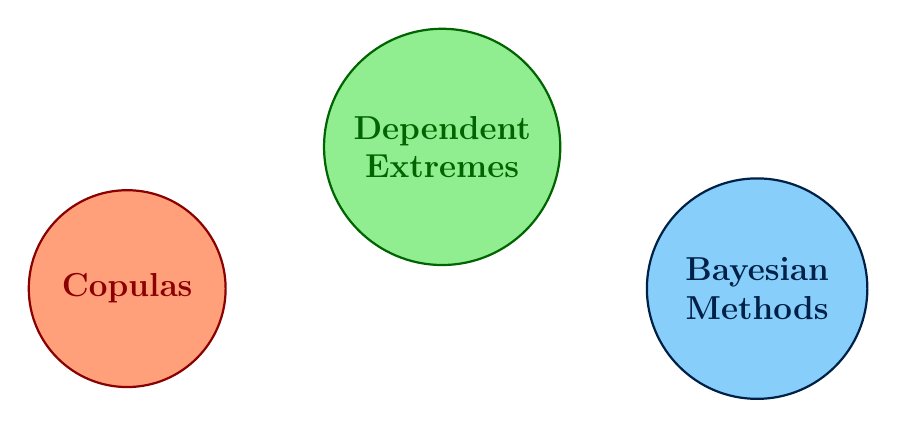
\begin{tikzpicture}[
    topic/.style={
        circle,
        draw,
        thick,
        minimum size=3cm,
        align=center,
        font=\large\bfseries
    }
]

% Center circle
\node[topic,
      fill=LightGreen,
      draw=DarkGreen,
      text=DarkGreen] (dep) at (0,0)
      {Dependent\\Extremes};

% Left lower circle
\node[topic,
      fill=LightSalmon,
      draw=DarkRed,
      text=DarkRed,
      minimum size=2.5cm] (cop) at (-4,-1.8)
      {Copulas};

% Right lower circle
\node[topic,
      fill=LightSkyBlue,
      draw=DarkBlue,
      text=DarkBlue,
      minimum size=2.8cm] (bayes) at (4,-1.8)
      {Bayesian\\Methods};

\end{tikzpicture}

\end{frame}

\begin{frame}{Starting Point: Copulas and Limit Distribution of the Maxima}
  Assume a univariate sequence $X_1, \dots , X_n$ has a common marginal distribution $F$, but the \alert{dependence} structure is given by an n-dimensional copula $C_n$, so that:
  \[
  P(X_1 \leq x_1, \dots, X_n \leq x_n) = C_n(F(x_1), \dots, F(x_n)).
  \] \pause

  Then, given the \alert{Distortion} $D(u) = \lim_{n \to \infty} \delta_n(u^{1/r_n})$, where $\delta_n$ is the copula \alert{diagonal} and $r_n$ a suitable rate function: \pause

  \[
  \lim_{n \to \infty} P \left(\frac{M_n - d^*_{\lceil{r_n}\rceil}}{c^*_{\lceil{r_n}\rceil}} \leq x \right) = D \circ H(x)
  \],

  where $M_n$ is the maximum of the sequence and $H$ is the GEV limiting distribution of the maximum for iid variables from $F$. See \parencite{herrmann2024}.
\end{frame}

\begin{frame}{Starting Goal and Related Problems}

  \begin{block}{Goal}
  \vspace{0.1cm}
    Estimate the limit distribution of the maxima
    \[
    D \circ H
    \]
    in order to infer the asymptotic behaviour of extremes.
  \end{block}

  \vspace{0.5cm}

  \begin{alertblock}{Challenges}
  \begin{itemize}
      \item Estimation of the $n$-dimensional copula.
      \item Potentially high-dimensional dependence structure.
      \item Only one realization of the univariate time series is observed.
  \end{itemize}
  \end{alertblock}

\end{frame}


\begin{frame}{Possible Directions}

% ===================== SLIDE 1: Block active =====================
\only<1>{

\begin{minipage}[t]{0.48\textwidth}

{\Large \textbf{Blocks Assumption}}

\vspace{0.3cm}

\begin{flushleft}
  \textcolor{green!60!black}{\checkmark} Replicates from the same copula allow inference on the copula structure \\
  \item \textcolor{red!70!black}{\texttimes} Strong assumption of copula stationarity
\end{flushleft}

\end{minipage}
\hfill
\begin{minipage}[t]{0.48\textwidth}

{\Large \textbf{\textcolor{gray}{Markov Assumption}}}

\vspace{0.3cm}

\begin{flushleft}
    \textcolor{gray}{\checkmark\ Existing Theory for Extremes of Markov Chains \parencite{winter2016}} \\
    \textcolor{gray}{\checkmark\ Copula Markov models already exist in the literature and are simple to estimate} \\
    \textcolor{gray}{\texttimes\ The connection to the theory of maxima becomes unclear}
\end{flushleft}

\end{minipage}
}

% ===================== SLIDE 2: Markov active =====================
\only<2>{

\begin{minipage}[t]{0.48\textwidth}

{\Large \textbf{\textcolor{gray}{Blocks Assumption}}}

\vspace{0.3cm}

\begin{flushleft}
  \textcolor{gray}{\checkmark\ Replicates from the same copula allow inference on the copula structure} \\
  \textcolor{gray}{\texttimes\ Strong assumption of copula stationarity}
\end{flushleft}

\end{minipage}
\hfill
\begin{minipage}[t]{0.48\textwidth}

{\Large \textbf{Markov Assumption}}

\vspace{0.3cm}

\begin{flushleft}
  \textcolor{green!60!black}{\checkmark} Existing Theory for Extremes of Markov Chains and applications \parencite{drees2015, winter2016} \\
   \textcolor{green!60!black}{\checkmark} Copula Markov models already exist in the literature and are simple to estimate \\
   \textcolor{red!70!black}{\texttimes} The connection to the theory of maxima becomes unclear
\end{flushleft}

\end{minipage}
}

\end{frame}

\begin{frame}{Copula Markov Chains}
  \begin{itemize}
    \item \textbf{Key Assumption}: $(X_{t-1}, X_t) \sim C(F(x_{t-1}), F(x_t))$
    \item \textbf{Properties}: Ergodicity and Mixing ($\beta$, $\rho$ mixing), \parencite{chen2009,longla2012}
    \item \textbf{Advantage:} If the common margin F is suited to model the entire distribution, we have a \alert{threshold-free} model for dependent extremes with a \alert{tail dependent} copula.
  \end{itemize}
\end{frame}

\begin{frame}{Extended GPD: Avoiding Threshold Selection}
    The idea is to transform the GPD by a suitable distortion function $G(u)$ \parencite{naveau2016}. \pause

    \begin{block}{Power Transformation}
      \vspace{0.1cm}
        For a random variable $X > 0$, the EGPD CDF is:
        \[
        F(x) = \left[ H_{\xi, \sigma}(x) \right]^\kappa
        \]
        where $H_{\xi, \sigma}(x)$ is the GPD CDF and \alert{$\kappa > 0$} is a bulk parameter.
    \end{block} \pause

    \textbf{Tail Consistency:} For any $\kappa > 0$, the tail behavior remains governed by $\xi$. The EGPD and GPD share the \alert{same extreme value index}.
\end{frame}

\begin{frame}{EGPD vs GPD: bulk change}
	\begin{figure}
		\centering
		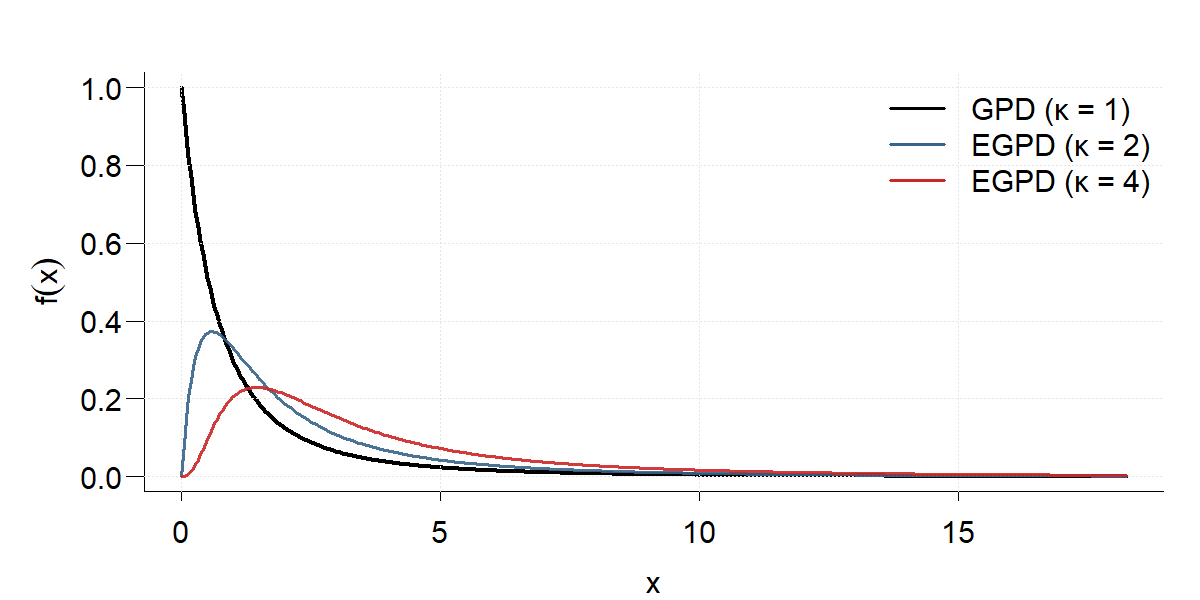
\includegraphics[width=\textwidth]{figures/egpd_plot.png}
	\end{figure}
\end{frame}

\begin{frame}{Copula Markov Chains: Simulation}
    \begin{block}{Sampling (Rosenblatt Transform)}
        \begin{enumerate}
            \item Generate $V_t \sim U(0,1)$
            \item Set $U_1 = V_1$ and $U_t = C^{-1}(V_t \mid U_{t-1})$ (Numerical Inversion)
            \item $X_t = F^{-1}(U_t)$
    \end{enumerate}
    \end{block}
\end{frame}

\begin{frame}{Simulation Example: EGPD(2,1,0.1) - Gumbel(4)}
    \begin{figure}
        \centering
        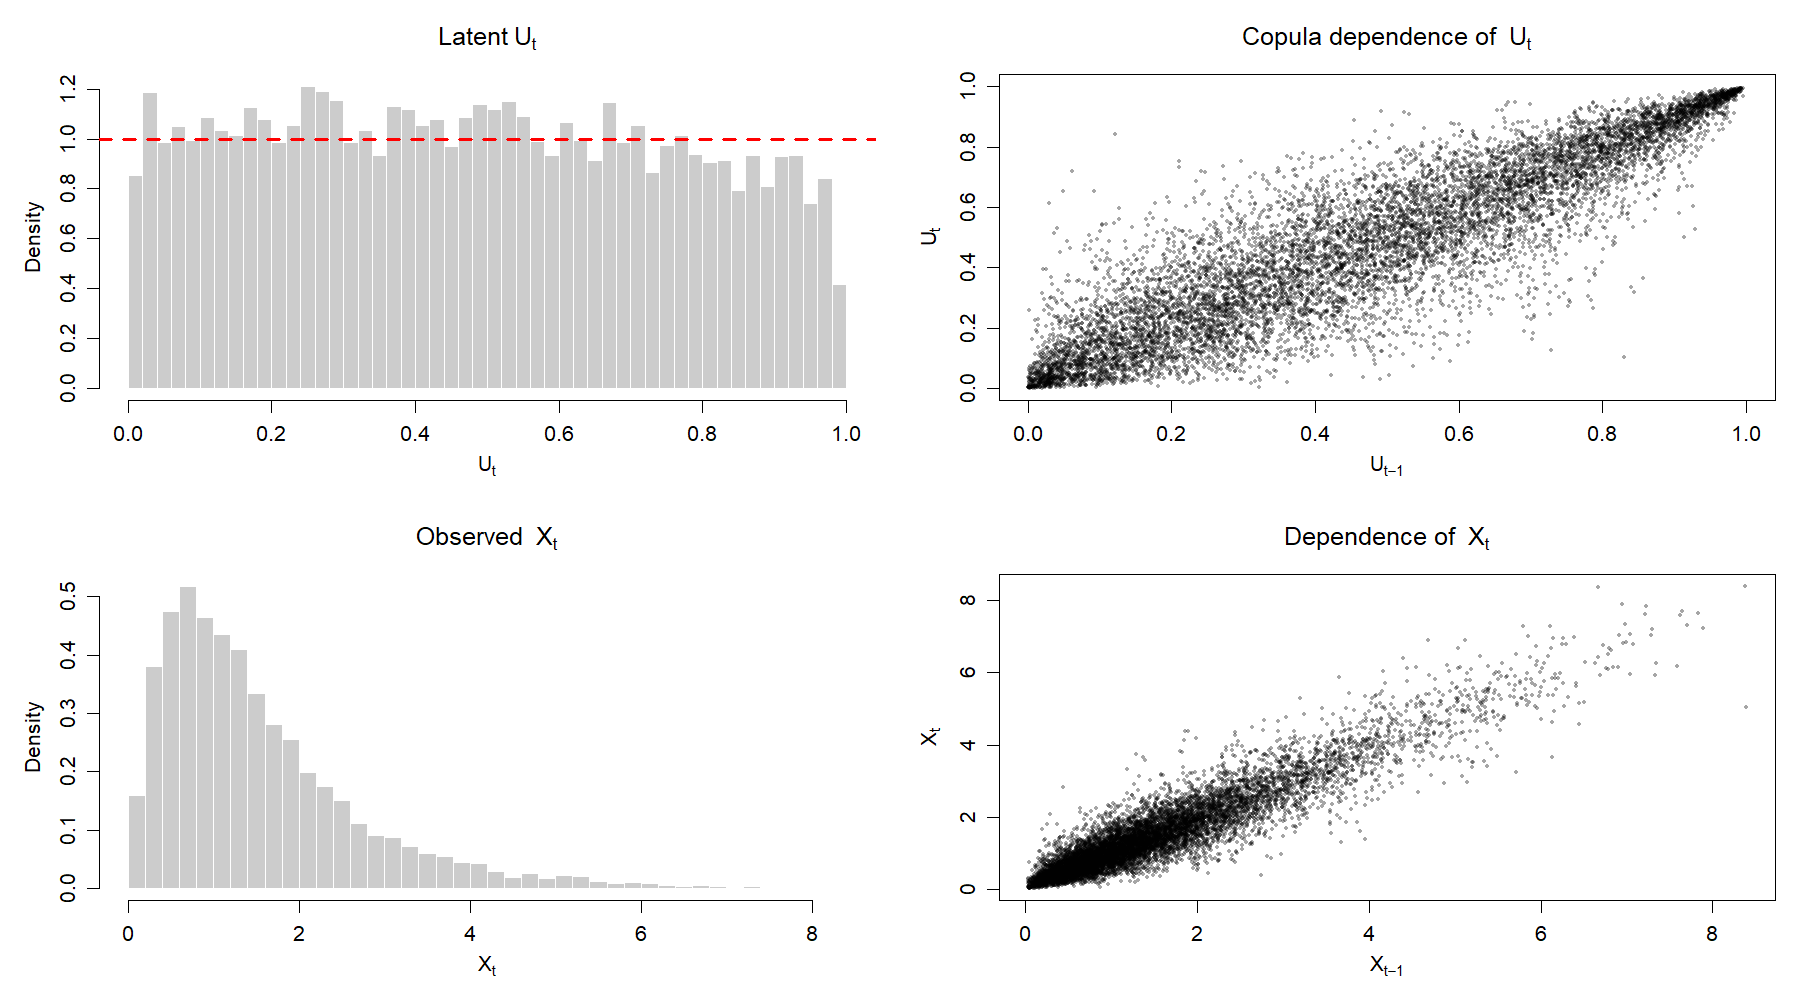
\includegraphics[width=\textwidth]{figures/copula_markov.png}
    \end{figure}
\end{frame}

\begin{frame}{Extreme Value Index: Speed of Convergence}
    \begin{figure}
            \centering
            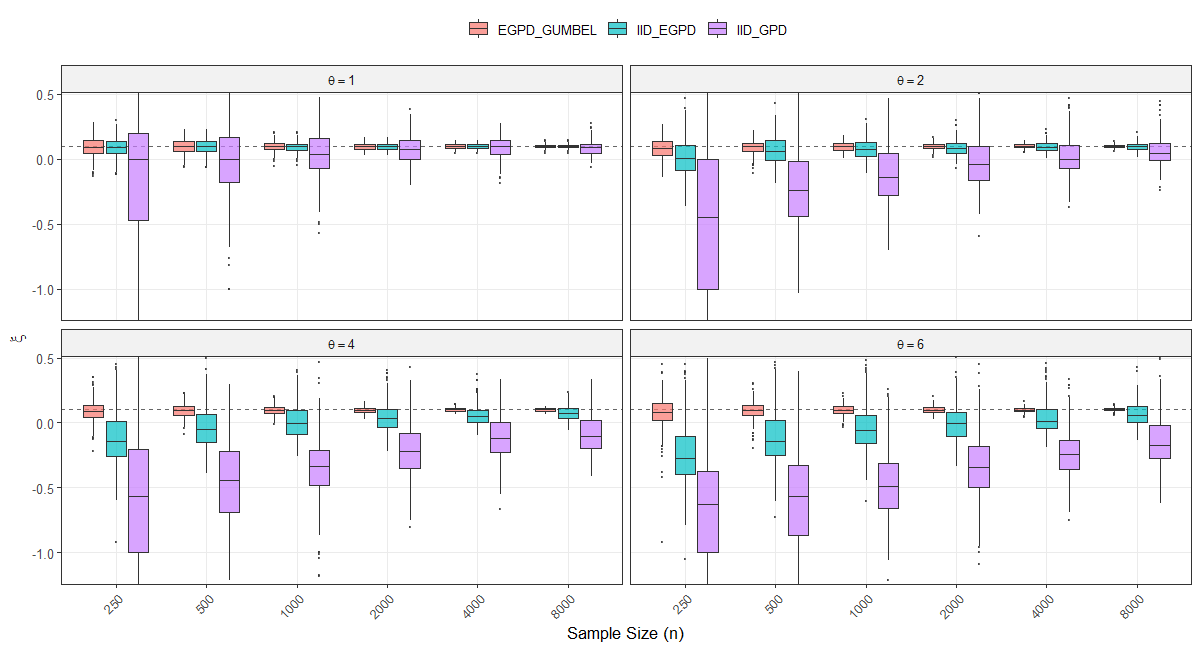
\includegraphics[width=\textwidth]{figures/sim_consistency1.png}
    \end{figure}
\end{frame}

\begin{frame}{Extreme Value Index: Copula Mispecification}
    \begin{figure}
        \centering
        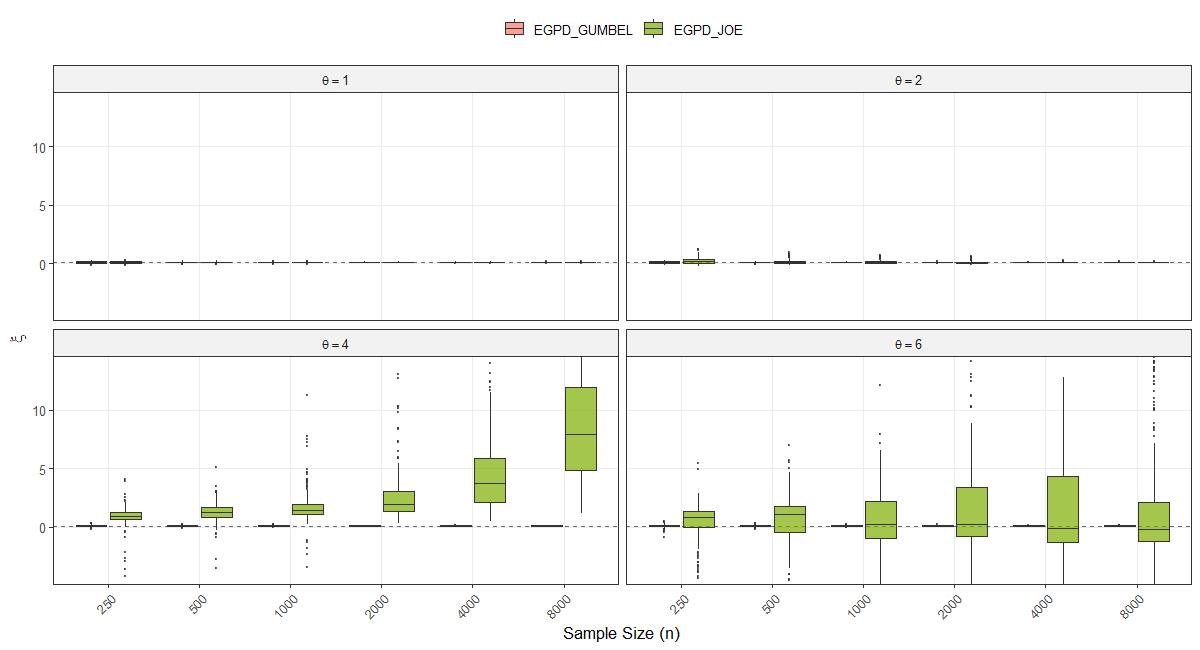
\includegraphics[width=\textwidth]{figures/sim_consistency4.png}
    \end{figure}
\end{frame}

\begin{frame}{Current Direction: More flexible dependence structure}
  \textbf{Question}: Can we construct Markov Chains with EGPD margin but not a fixed Copula structure for the transitions?

  Current ideas:
  
  \begin{itemize}
    \item Dynamic Copula Mixtures \parencite{andre2024}
    \item Multivariate EGPD \parencite{gaetan2025}
  \end{itemize}
\end{frame}

\begin{frame}[allowframebreaks, noframenumbering]
  \printbibliography
\end{frame}

\end{document}